\section{Espelhos de Corrente}

Espelhos de Corrente foram necess\'arios para o desenvolvimento de diversos blocos contidos no projeto, e ser\~ao especificados nas subse{\c c}\~oes \` seguinte. Uma explica{\c c}\~ao geral sobre o funcionamento e desenvolvimento de espelhos de corrente pode ser visto na \autoref{anexoespelhos}.

\newcommand{\NomeBloco}{NULL}
\newcommand{\NomeBlocoNoUnderline}{NULL}
\newcommand{\NomePTab}{tab_\NomeBlocoNoUnderline}
\newcommand{\NomeSTab}{tab_\NomeBlocoNoUnderline2}
\newcommand{\NomePFig}{fig_\NomeBlocoNoUnderline}
\newcommand{\NomeSFig}{fig_\NomeBlocoNoUnderline2}
\newcommand{\NomeTTab}{tab_\NomeBlocoNoUnderline3}
\newcommand{\NomeQTab}{tab_\NomeBlocoNoUnderline4}

\renewcommand{\NomeBloco}{ibias\_generator}
\renewcommand{\NomeBlocoNoUnderline}{ibiasgenerator}
\renewcommand{\NomePTab}{tab_\NomeBlocoNoUnderline}
\renewcommand{\NomeSTab}{tab_\NomeBlocoNoUnderline2}
\renewcommand{\NomePFig}{fig_\NomeBlocoNoUnderline}
\renewcommand{\NomeSFig}{fig_\NomeBlocoNoUnderline2}
\renewcommand{\NomeTTab}{tab_\NomeBlocoNoUnderline3}
\renewcommand{\NomeQTab}{tab_\NomeBlocoNoUnderline4}

\subsection{ibias\_generator}
 
O bloco \NomeBloco{}\footnote{Circuito desenvolvido pelo aluno \textit{Daniel Carvalho Lott}, do curso de bacharelado em Engenharia Elétrica da UFMG, no ano de 2020} \'e um espelho de corrente que apresenta uma sa\'ida de 50 $\mu$A. O bloco apresenta as definições de sinais de entrada e sa\'ida referidos na \autoref{\NomeSTab}.

\begin{table}[htbp]
\caption{Sinais do bloco \NomeBloco}
\label{\NomeSTab}
\centering
\begin{tabular}{ccl}

    \toprule
    Sinal & Tipo    & Descrição        \\
    \midrule \midrule
    ibias\_1   & Saída   & Fonte de Corrente de 50 $\mu$A \\
    \bottomrule
\end{tabular}
\legend{Fonte: Produzido pelo autor}
\end{table}

O circuito projetado para o bloco \'e demonstrado na \autoref{\NomePFig}.

\begin{figure}[htb]
 \centering
    \centering
    \caption{Circuito CMOS projetado para o bloco \NomeBloco} 
    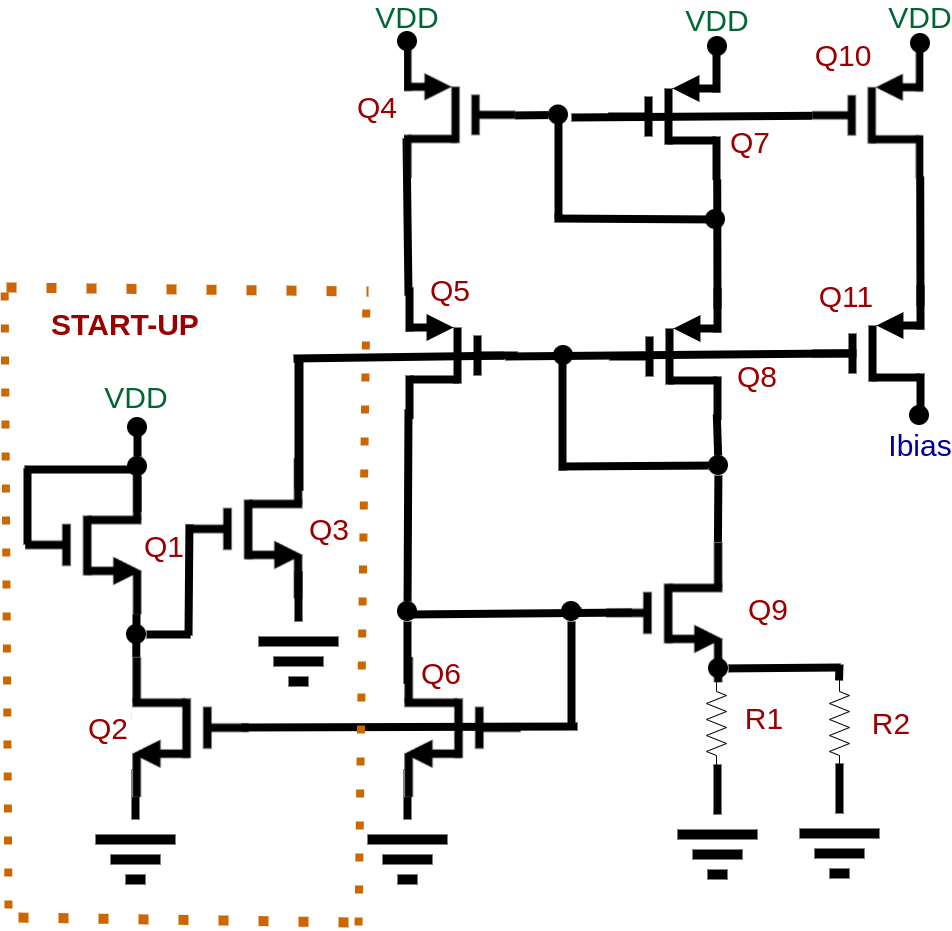
\includegraphics[scale=0.3]{Circuitos/Ibias_generator.png}
    \legend{Fonte: Produzido pelo autor}
    \label{\NomePFig}
\end{figure}

\begin{figure}[htb]
 \centering
    \centering
    \caption{Representação em bloco do \NomeBloco} \label{\NomeSFig}
    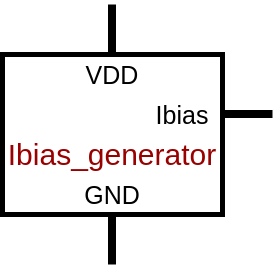
\includegraphics[scale=0.3]{Circuitos/ibias_generator_block.png}
    \legend{Fonte: Produzido pelo autor}
\end{figure}

Os transistores utilizados no bloco apresentam os par\^ametros mostrados na \autoref{\NomeTTab}.

\begin{table}[htbp]
\caption{Transistores do Bloco \NomeBloco}
\label{\NomeTTab}
\centering
\begin{tabular}{ccccc}
\toprule
Transistor & W ($\mu$m)  & L ($\mu$m)           & M (n° dispositivos) & S (n° dispositivos)\\
\midrule \midrule
Q1 & 0,3 & 19,995 & 1 & 3\\
\midrule
Q2 & 25 & 0,5 & 2 & 1\\
\midrule
Q3 & 30 & 0,5 & 1 & 1\\
\midrule
Q4, Q7 e Q10 & 35 & 4 & 2 & 1\\
\midrule
Q5, Q8 e Q11 & 25 & 2,5 & 2 & 1\\
\midrule
Q6 & 20 & 4 & 2 & 1\\
\midrule
Q9 & 20 & 4 & 4 & 1\\
\midrule
Q10 & 25 & 2,5 & 2 & 1\\
\midrule
Q11 & 25 & 2,5 & 2 & 1\\
\bottomrule
\end{tabular}
\legend{Fonte: Produzido pelo autor}
\end{table}

O resistor utilizado no bloco apresenta os par\^ametros mostrados na \autoref{\NomeQTab}.

\begin{table}[htbp]
\caption{Resistor do bloco \NomeBloco}
\label{\NomeQTab}
\centering
\begin{tabular}{ccccc}
\toprule
Resistor & W ($\mu$m)  & L ($\mu$m) & M (n° dispositivos) & Resist\^encia (k$\Omega$)\\
\midrule \midrule
R & 8 & 29,98 & 2 & 0,569025\\
\bottomrule
\end{tabular}
\legend{Fonte: Produzido pelo autor}
\end{table}

Os transistores \textit{Q6} e \textit{Q9}, juntos aos resistores \textit{R1} e \textit{R2}, t\^em a finalidade de funcionarem como um dreno de corrente referenciados pelos resistores. Os transistores \textit{Q4} e \textit{Q7} t\^em a finalidade de funcionarem como uma fonte de corrente, referenciados pelo dreno de corrente j\'a mencionado. O transistor \textit{Q10} \'e o braço do espelho de corrente do qual fornece a corrente de sa\'ida.

Os transistores \textit{Q5}, \textit{Q8} e \textit{Q11} se apresentam na configuração \textit{Cascode}, que tem o intuito de tornar o espelho de corrente de resposta mais linear, aumentar sua banda e ainda aumentar as suas resist\^encias de entrada e sa\'ida.

Os transistores \textit{Q1}, \textit{Q2} e \textit{Q3} t\^em a função de inicializar o circuito no ponto de operação adequado, j\'a que o circuito tamb\'em apresenta estabilidade quando fornecendo 0 A, sendo necess\'ario evitar essa situação.

\renewcommand{\NomeBloco}{\textit{iref\_generator}}
\renewcommand{\NomeBlocoNoUnderline}{irefgenerator}
\renewcommand{\NomePTab}{tab_\NomeBlocoNoUnderline}
\renewcommand{\NomeSTab}{tab_\NomeBlocoNoUnderline2}
\renewcommand{\NomePFig}{fig_\NomeBlocoNoUnderline}
\renewcommand{\NomeSFig}{fig_\NomeBlocoNoUnderline2}
\renewcommand{\NomeTTab}{tab_\NomeBlocoNoUnderline3}
\renewcommand{\NomeQTab}{tab_\NomeBlocoNoUnderline4}

\subsection{iref\_generator}

O bloco \NomeBloco{}\footnote{Circuito desenvolvido por \textit{Dalton Martini Colombo}, orientador do trabalho aqui apresentado} \'e um espelho de corrente que apresenta algumas sa\'idas como fonte e outras em dreno de corrente. O bloco apresenta as definições de sa\'ida referidos na \autoref{\NomeSTab}.

\begin{table}[!h]
\caption{Sinais do bloco \NomeBloco}
\label{\NomeSTab}
\centering
\begin{tabular}{ccl}

    \toprule
    Sinal & Tipo    & Descrição        \\
    \midrule \midrule
    iref1\_src   & Saída   & Fonte de Corrente de 0.5 $\mu$A \\
    \midrule
    iref2\_src   & Saída   & Fonte de Corrente de 0.5 $\mu$A \\
    \midrule
    iout\_test   & Saída   & Fonte de Corrente de 1.5 $\mu$A \\
    \midrule
    iref1\_sink   & Saída   & Dreno de Corrente de 0.5 $\mu$A \\
    \midrule
    iref2\_sink   & Saída   & Dreno de Corrente de 0.5 $\mu$A \\
    \bottomrule
\end{tabular}
\legend{Fonte: Produzido pelo autor}
\end{table}

O circuito projetado para o bloco \'e demonstrado na \autoref{\NomePFig}.

\begin{figure}[htb]
 \centering
    \centering
    \caption{Circuito CMOS projetado para o bloco \NomeBloco} 
    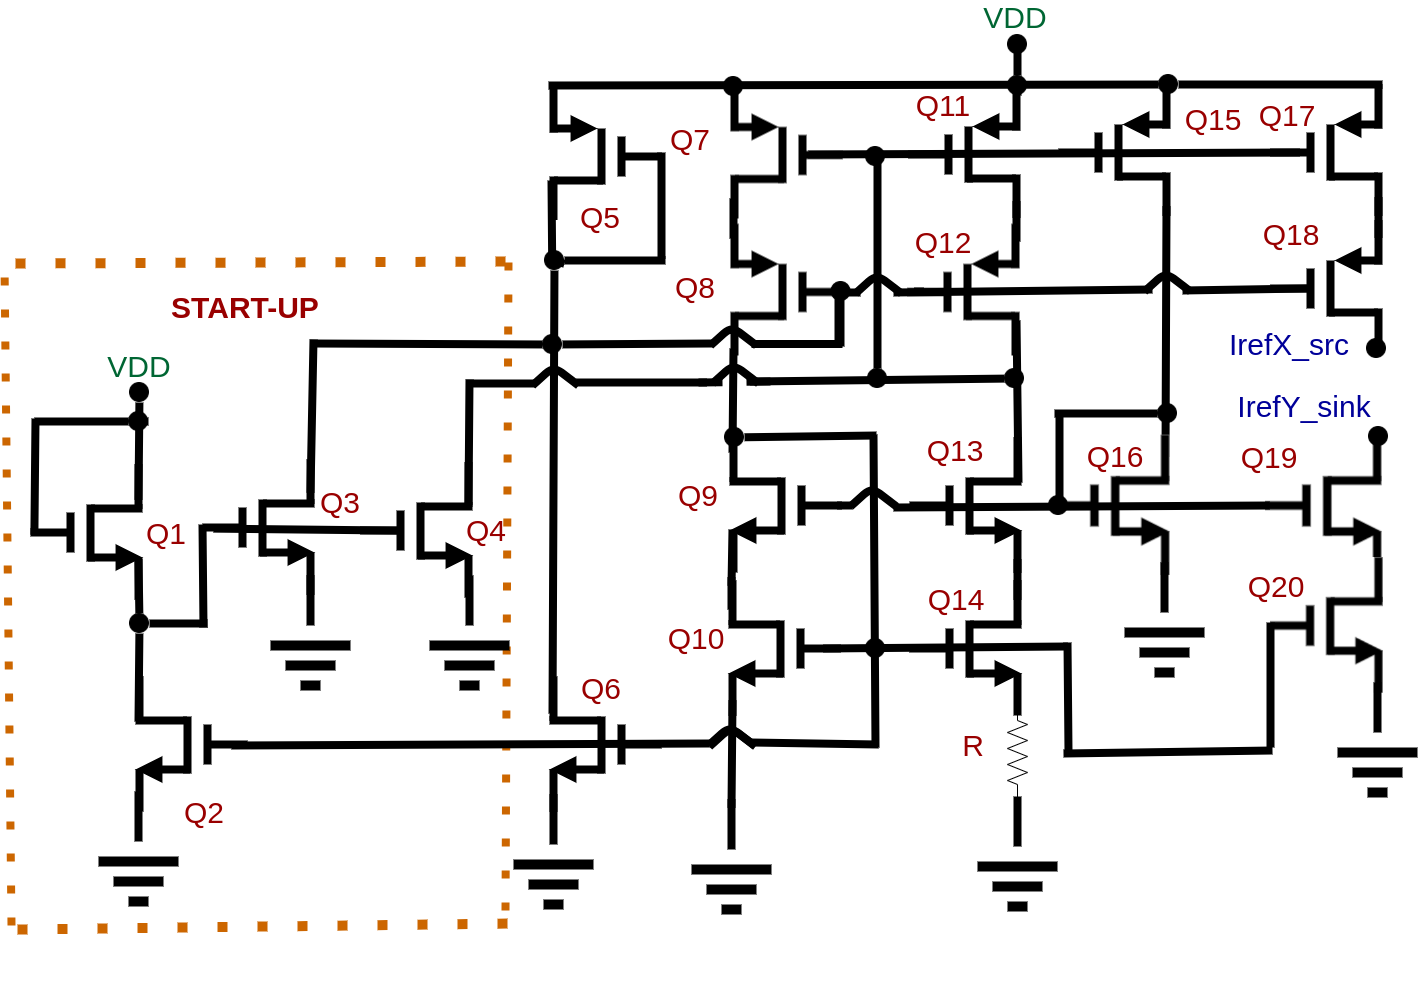
\includegraphics[scale=0.3]{Circuitos/iref_generator.png}
    \legend{Fonte: Produzido pelo autor}
    \nota{Nem todos transistores são representados na imagem. \emph{Q17}, \emph{Q18}, \emph{Q19} e \emph{Q20} são transistores replicados para cada sa\'ida \emph{IrefX\_src} e \emph{IrefY\_sink}, onde \emph{X} e \emph{Y} são os identificadores de cada sa\'ida}
    \label{\NomePFig}
\end{figure}

\begin{figure}[htb]
 \centering
    \centering
    \caption{\label{\NomeSFig}Representação em bloco do \NomeBloco}
    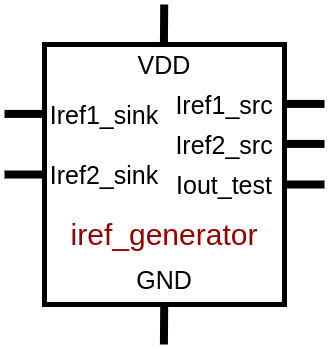
\includegraphics[scale=0.3]{Circuitos/iref_generator_block.png}
    \legend{Fonte: Produzido pelo autor}
\end{figure}

Os transistores utilizados no bloco apresentam os par\^ametros mostrados na \autoref{\NomeTTab}.

\begin{table}[!h]
\caption{Transistores do Bloco \NomeBloco}
\label{\NomeTTab}
\centering
\begin{tabular}{ccccc}
\toprule
Transistor & W ($\mu$m)  & L ($\mu$m)  & M (n° dispositivos) & S (n° dispositivos)\\
\midrule \midrule

\midrule
Q1                                   & 0,3    & 19,995 & 1                   & 3                   \\
\midrule
Q2                                   & 35     & 0,18   & 2                   & 1                   \\
\midrule
Q3 e Q4                              & 15     & 0,18   & 1                   & 1                   \\
\midrule
Q5                                   & 10     & 15     & 1                   & 6                   \\
\midrule
\begin{tabular}[c]{@{}c@{}}Q6, Q9, Q10,\\ Q13, Q19 e Q20\end{tabular}          & 4      & 19,995 & 1                   & 2                   \\
\midrule
\begin{tabular}[c]{@{}c@{}}Q7, Q8, Q11, Q12,\\ Q15, Q17a¹ e Q18a¹\end{tabular} & 10     & 15   & 2                   & 1                   \\
\midrule
Q14                                  & 4      & 19,995 & 10                  & 1                   \\
\midrule
Q16                                  & 4      & 19,995 & 1                   & 6 \\
\midrule
Q17b² e Q18b²                                                                  & 10     & 15     & 6                   & 1                  \\
\bottomrule
\end{tabular}
\legend{Fonte: Produzido pelo autor}
\legend{¹ Q17a e Q18a são os transistores referentes \`as sa\'idas iref1\_src e iref2\_src\\
² Q17b e Q18b são os transistores referentes \`a sa\'ida iout\_test}
\end{table}

O resistor \emph{R} utilizado no bloco apresenta os par\^ametros mostrado na \autoref{\NomeQTab}.

\begin{table}[!h]
\caption{Resistores do bloco \NomeBloco}
\label{\NomeQTab}
\centering
\begin{tabular}{cccc}
\toprule
Resistor & W ($\mu$m)  & L ($\mu$m) & Resist\^encia (k$\Omega$)\\
\midrule \midrule
R & 3 & 404,4 & 141,996\\
\bottomrule
\end{tabular}
\legend{Fonte: Produzido pelo autor}
\end{table}

Os transistores \emph{Q6} e \emph{Q9}, juntos aos resistores \emph{R1} e \emph{R2}, t\^em a finalidade de funcionarem como um dreno de corrente referenciados pelos resistores. Os transistores \emph{Q4} e \emph{Q7} t\^em a finalidade de funcionarem como uma fonte de corrente, referenciados pelo dreno de corrente j\'a mencionado. O transistor \emph{Q10} \'e o braço do espelho de corrente do qual fornece a corrente de sa\'ida.

Os transistores \emph{Q5}, \emph{Q8} e \emph{Q11} se apresentam na configuração \emph{Cascode}, que tem o intuito de tornar o espelho de corrente de resposta mais linear, aumentar sua banda e ainda aumentar as suas resist\^encias de entrada e sa\'ida.

Os transistores \emph{Q1}, \emph{Q2} e \emph{Q3} t\^em a função de inicializarem o circuito no ponto de operação adequado, j\'a que o circuito tamb\'em apresenta estabilidade quando fornecendo 0 A, sendo necess\'ario evitar essa situação.

\renewcommand{\NomeBloco}{current\_mirror\_nmos}
\renewcommand{\NomeBlocoNoUnderline}{curmirnmosb}
\renewcommand{\NomePTab}{tab_\NomeBlocoNoUnderline}
\renewcommand{\NomeSTab}{tab_\NomeBlocoNoUnderline2}
\renewcommand{\NomePFig}{fig_\NomeBlocoNoUnderline}
\renewcommand{\NomeSFig}{fig_\NomeBlocoNoUnderline2}
\renewcommand{\NomeTTab}{tab_\NomeBlocoNoUnderline3}
\renewcommand{\NomeQTab}{tab_\NomeBlocoNoUnderline4}

\subsubsection{\NomeBloco}

O bloco \NomeBloco{} cont\'em alguns bra{\c c}os utilizados como dreno de corrente para outras partes do circuito, sendo todos valores iguais \'a corrente de refer\^encia. O bloco apresenta as defini{\c c}\~oes de sinais de entrada e sa\'ida referidos na \autoref{\NomeSTab}.

\begin{table}[htbp]
\caption{Sinais do bloco \NomeBloco}
\label{\NomeSTab}
\centering
\begin{tabular}{ccl}

    \toprule
    Sinal & Tipo    & Descri{\c c}\~ao        \\
    \midrule \midrule
    Iref\_bias   & Entrada   &  Corrente de refer\^encia para os bra{\c c}os \\
    \midrule
    Iref\_A   & Saída   &  Bra{\c c}o 1 \\
    \midrule
    Iref\_B   & Saída   &  Bra{\c c}o 2 \\
    \midrule
    Iref\_C   & Saída   &  Bra{\c c}o 3 \\
    \midrule
    Iref\_D   & Saída   &  Bra{\c c}o 4 \\
    \midrule
    Iref\_E   & Saída   &  Bra{\c c}o 5 \\
    \bottomrule
\end{tabular}
\legend{Fonte: Produzido pelo autor}
\end{table}

O circuito projetado para o bloco \'e demonstrado na \autoref{\NomePFig}.

\begin{figure}[htb]
 \centering
    \centering
    \caption{Circuito CMOS projetado para o bloco \NomeBloco} 
    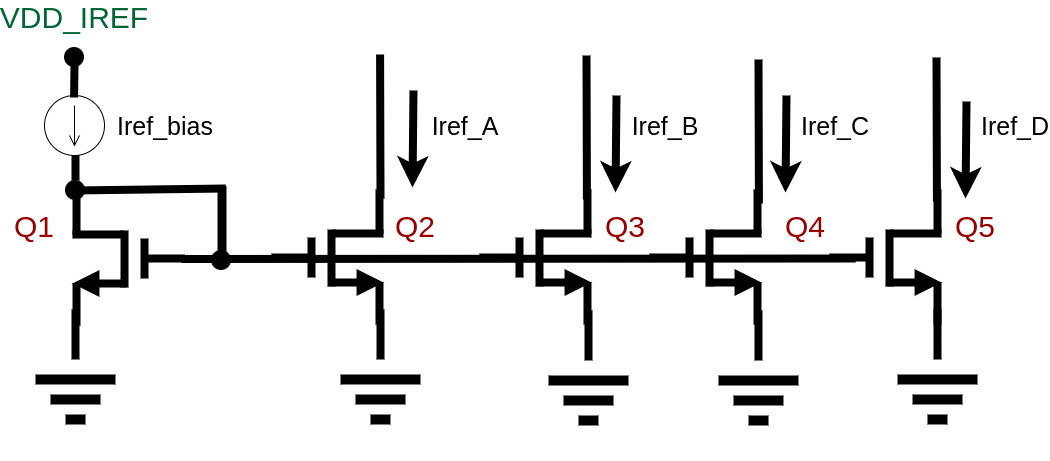
\includegraphics[scale=0.3]{Circuitos/current_mirror.png}
    \legend{Fonte: Produzido pelo autor}
    \label{\NomePFig}
\end{figure}

\begin{figure}[htb]
 \centering
    \centering
    \caption{Representa{\c c}\~ao em bloco do \NomeBloco} \label{\NomeSFig}
    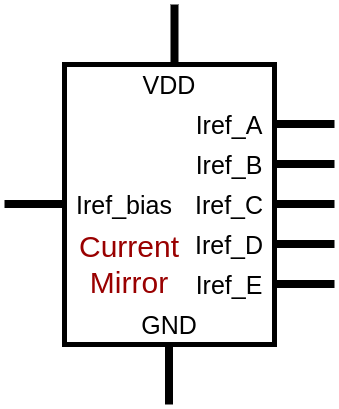
\includegraphics[scale=0.3]{Circuitos/current_mirror_block.png}
    \legend{Fonte: Produzido pelo autor}
\end{figure}

Os transistores utilizados no bloco \NomeBloco{} apresentam os par\^ametros mostrados na \autoref{\NomeTTab}.

\begin{table}[htbp]
\caption{Transistores do Bloco \NomeBloco}
\label{\NomeTTab}
\centering
\begin{tabular}{ccccc}
\toprule
Transistor & W ($\mu$m)  & L ($\mu$m)           & M (n° dispositivos) & S (n° dispositivos)\\
\midrule \midrule
\begin{tabular}[c]{@{}c@{}}Q1, Q2, Q3,\\
Q4, Q5 e Q6\end{tabular} & 5 & 6 & 2 & 1\\
\bottomrule
\end{tabular}
\legend{Fonte: Produzido pelo autor}
\end{table}
